\chapter{Bildvorverarbeitung \dcfirstauthorshort}
\label{cha:bildvorverarbeitung}

% Überblick
\begin{figure}[ht] % [htb]
	\centering
	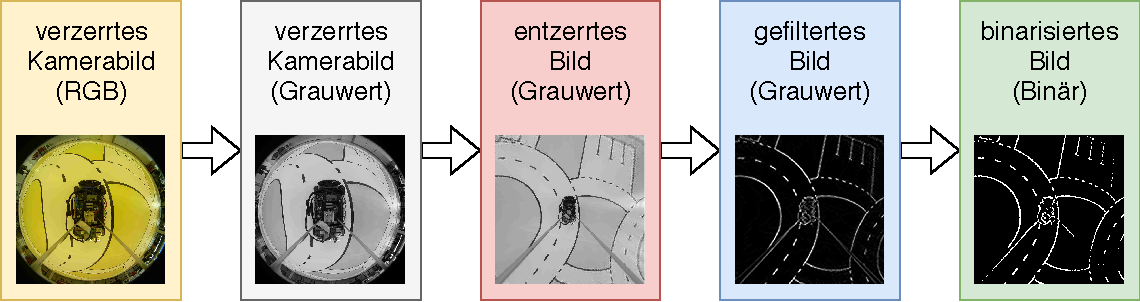
\includegraphics[width=1\textwidth]{bildvorverarbeitung_ueberblick.pdf}
	\caption{Schritte in der Bildvorverarbeitung}
	\label{fig:bildvorverarbeitung_ueberblick}
\end{figure} 

Ein Bild ist eine Matrix aus Punkten, denen ein Farbwert zugeordnet wird. In der Bildverarbeitung gilt es in diesen farbigen Punkten enthaltene Informationen zu extrahieren. Der einzige uns zur Verfügung stehende Sensor ist neben den Radencodern und der \gls{acr:imu} die in Vogelperspektive montierte Fischaugenkamera. Ziel nach der Aufnahme des Bildes ist es, Auskunft über die Position von Fahrspurmarkierungen zu erhalten, damit weitere Algorithmen (in Kapitel~\ref{cha:fahrspurerkennung} beschrieben) daraus die für die Regelung relevanten Punkte detektieren können. Letztlich werden die Pixel gesucht, welche einer Linie zugehörig sind. Der menschliche Betrachter des Bildes erkennt die Linie sofort. Für die automatisierte Extraktion von Markierungspunkten bedarf es jedoch einer dem Rechner verständlichen Definition, wann ein Pixel einer Linie zugehörig ist. Dafür werden Linienpunkte durch die folgend beschriebenen Bildvorverarbeitungsschritte hervorgehoben, damit das Kriterium für den Rechner lautet: Alle Pixel, welche heller als ein bestimmter Schwellwert sind, gehören zu den Fahrbahnmarkierungspunkten. Zum Überblick sind die Verarbeitungsstufen vom Rohbild bis zum Endergebnis in Abbildung~\ref{fig:bildvorverarbeitung_ueberblick} dargestellt.

\section{Bildentzerrung}

Der große Vorteil des Fischaugenobjektivs ist es, Bereiche in größerer Entfernung aller Richtungen wahrnehmen zu können. Andererseits ist das Bild aufgrund des enormen Weitwinkels stark verzerrt. Zur Erstellung einer Weltkarte ist es daher sinnvoll, dessen Verzerrung zu rektifizieren. Dazu wurde sich in MATLAB wie in Kapitel~\ref{sec:kameramodell} beschrieben der \gls{acr:ocamcalib}-Toolbox bedient. Da die Farbinformationen der Rohdaten keine Anwendung finden und sowohl die Toolbox als auch die Faltungsfilter lediglich mit Graustufenbildern arbeiten können, erfolgt vor der Entzerrung eine Umwandlung in ein Graustufenbild.

% Das ver- und entzerrte Bild nebeneinander
\begin{figure}[ht] % [htb]
  \centering
  \subfloat[][]{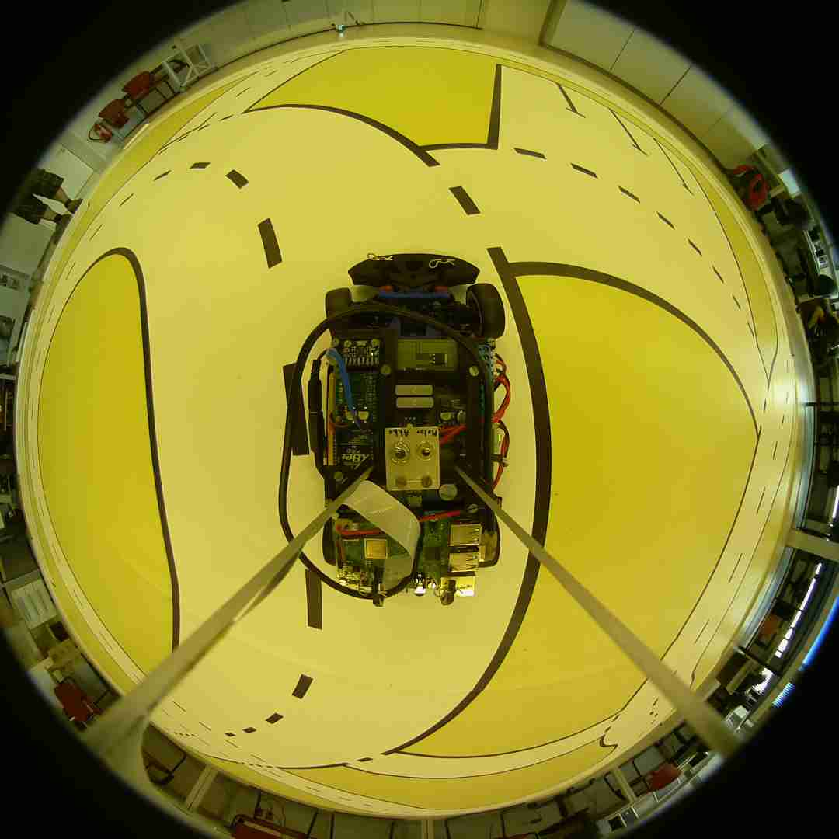
\includegraphics[width=0.45\textwidth]{bildvorverarbeitung_fischauge.png}}
  \qquad
  \subfloat[][]{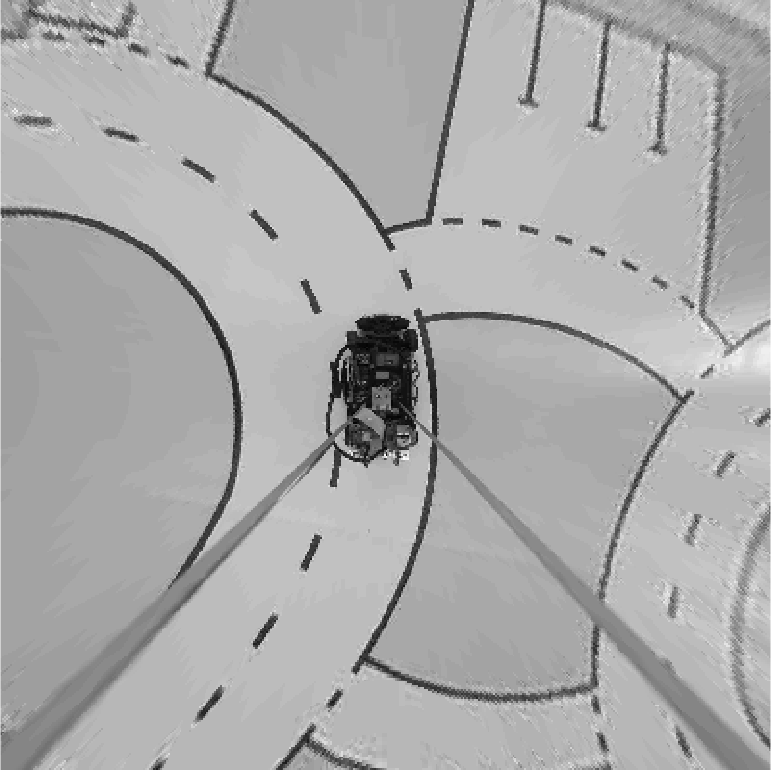
\includegraphics[width=0.45\textwidth]{bildvorverarbeitung_entzerrt.png}}
%  \includegraphics[width=0.9\textwidth]{bildvorverarbeitung_entzerren.png}
  \caption{verzerrtes Rohbild (a) und entzerrtes Graustufenbild (b) einer Momentaufnahme im Parcours}
\label{fig:bildvorverarbeitung_entzerren}
\end{figure} 

\subsection{Festlegung der Auflösung}
In Abbildung~\ref{fig:bildvorverarbeitung_entzerren} ist ein Bild original (links) und nach der Entzerrung (rechts) zu sehen. Im entzerrten Bild fällt auf, dass zum Rand die Auflösung durch dessen Transformation zunehmend schlechter wird. Diese Tatsache lässt den Schluss zu, für die Kamera die vorzugsweise vollste Auflösung zu wählen, mit dem Ziel, die Informationsdichte am Bildrand so hoch wie möglich zu halten. Damit einher geht allerdings eine längere Übertragungszeit des Bildes vom Roboter zum Rechner. Um diese Zeit durchführbar gering zu halten, gilt es die niedrigste Auflösung bei möglichst uneingeschränkter Funktionalität zu bestimmen. 

Das dafür entscheidende Kriterium ist das kleinste, zu detektierende Objekt, welches in seiner Größe zwei Pixel nicht unterschreiten darf. In unserem Fall ist dies die Breite einer Fahrbahnmarkierung im entzerrten Bild. Aus Sicherheitsgründen ist die Auflösung nach der Entzerrung mit 400\( \times \)400 Pixeln so gewählt, dass die Spurmarkierung eine Dicke von ca. 4-6 Pixeln aufweist. 

Durch die als ausreichend festgelegte Sichtweite ergibt sich die Auflösung des verzerrten Kamerabildes. Sie wurde empirisch auf 1080\( \times \)1080 so eingestellt, dass nach der Filterung des entzerrten Bildausschnitts alle Linien bis zum Rand akzeptabel erkennbar geblieben sind.

\section{Filterung}
\label{sec:bildvorverarbeitung:filterung}
Die Aufnahme kann nun wie in Kapitel~\ref{sec:filter} beschrieben gefiltert werden, damit sich die Kanten (sprich: steile Übergänge von hellen zu dunklen Pixeln oder andersherum) hervorheben. Monotone Bildbereiche sollen dunkel bleiben. Unter Durchführung einer Kantendetektion auf dem entzerrten Bild erhielte man sehr viele Treffer, da durch sensorbedingtes Bildrauschen den Kantendetektor ansprechende Störungen enthalten sind. 

Das in Abbildung~\ref{fig:bildvorverarbeitung_filtern} (a) dargestellte Filterergebnis wurde mit einem \gls{acr:log}-Filter erzielt. Dieser vereint mit der gaußschen Glättung und dem Laplace-Operator die Ausführung zweier Filter. Wie in Abschnitt~\ref{ssec:laplaceFilter} erklärt, stellen Kanten in der Filterantwort die Nulldurchgänge zwischen den positiven und negativen Peaks dar. Da das gefilterte Bild keine Pixelwerte kleiner Null zugewiesen bekommt, sind nur deren stark positiven Anstiegsänderungen (2. Ableitung \( > 0\)) in Abb.~\ref{fig:bildvorverarbeitung_filtern} (a) sichtbar. 

Im Allgemeinen treten an einer Linie zwei Kanten auf. Jedoch lassen sich mit entsprechend eingestellten Parameterwerten die zwei an jeder Fahrbahnmarkierung entstandenen positiven Peaks zu einer sichtbaren, die Fahrbahnbegrenzung repräsentierenden, hellen Linie verwischen. 

Um wertvolle Rechenzeit während der aufwändigen Filterung einzusparen, werden das Bild mit je einem eindimensionalen 15\( \times \)1 bzw. 1\( \times \)15 Filter in \( {\gls{x}}^{\gls{lat:BildKOS}} \)- und \( {\gls{y}}^{\gls{lat:BildKOS}} \)-Richtung verarbeitet und anschließend die Filterergebnisse addiert. Diese Alternative zu der in Abschnitt~\ref{sec:filter} beschriebenen Separierbarkeit hat ebenfalls einen deutlich schnelleren Funktionsablauf ermöglicht. Erstaunlicherweise ist die Qualität des gefilterten Bildes sehr gut, sodass die Weiterverarbeitung verlässliche Informationen liefert.


% Das gefilterte und binarisierte Bild nebeneinander
\begin{figure}[hb] % [htb]
  \centering
  \subfloat[][]{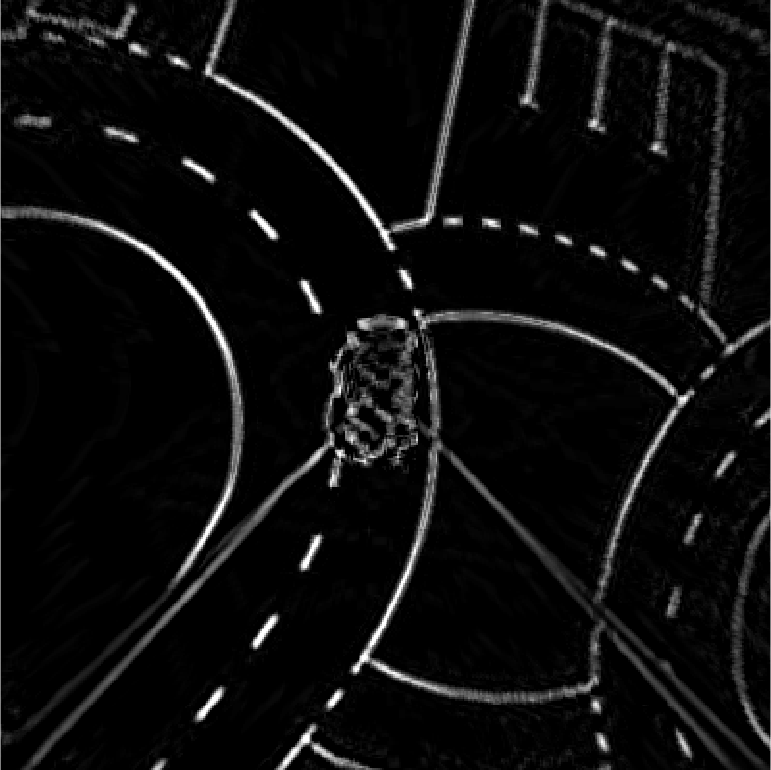
\includegraphics[width=0.45\textwidth]{bildvorverarbeitung_gefiltert.png}}
  \qquad
  \subfloat[][]{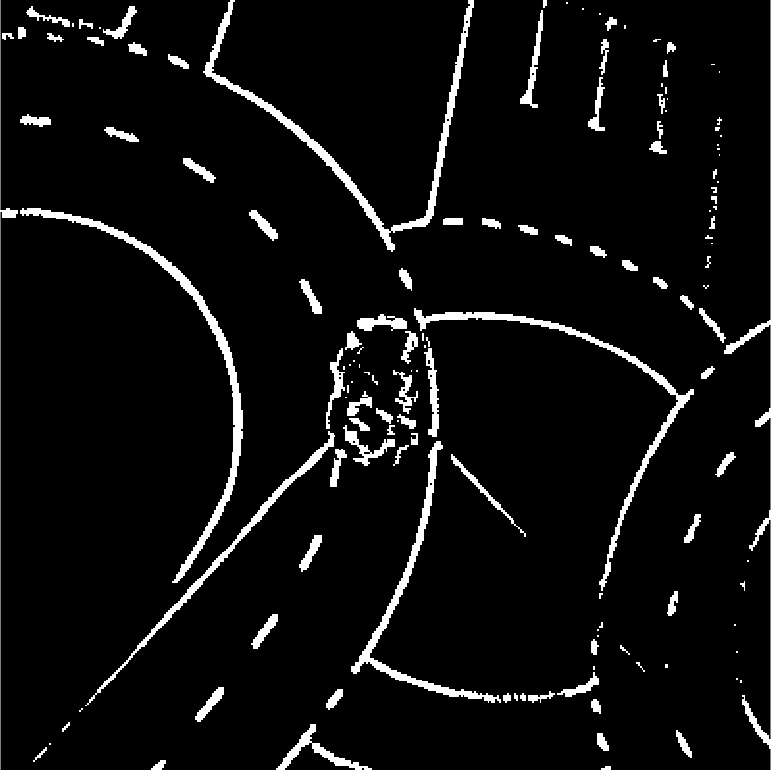
\includegraphics[width=0.45\textwidth]{bildvorverarbeitung_binarisiert.png}}
  \caption{gefiltertes (a) und anschließend binarisiertes Bild (b) einer Momentaufnahme im Parcours}
\label{fig:bildvorverarbeitung_filtern}
\end{figure} 

\section{Binarisierung}
\label{sec:bildvorverarbeitung:binarisierung}
Der Schwellwert, welcher entscheidet, ob ein Pixel im binarisierten Bild den Wert \glqq \(0\)\grqq{} oder\glqq \(1\)\grqq{} erhält, wurde fest als Parameter eingestellt. Dessen Ermittlung ging aus der empirischen, manuellen Sichtprüfung in Abstimmung der Filterparameter hervor. Alle weiteren Bildverarbeitungsalgorithmen ziehen das binarisierte oder gefilterte Bild als Grundlage ihrer Berechnungen heran.